\chapter{Reconstrucci\'on de los eventos  y selecci\'on de eventos candidatos}
\label{ch:selAuger}

En este capítulo se describe la metodología aplicada para elegir el criterio de selección en las tres búsquedas.
En primer lugar se definen cortes de calidad que eliminan estaciones o incluso eventos espúreos, con el fin de lograr una reconstrucción confiable.
Una vez hecho esto se utilizan variables topológicas y temporales para elegir eventos inclinados, y luego  se agrega información de las trazas para seleccionar las lluvias jóvenes.

\section{Criterios de calidad}

	Al inicio de la cadena de procesamiento se cuenta con un conjunto de eventos que cumplen el criterio de trigger T3.
	De este grupo, se eliminan en primer lugar los datos que se hayan tomado en períodos en los que el detector se haya comportado de manera inestable.
	Luego, se aplica a cada evento una serie de procedimientos que se mencionan a continuación:
	\begin{itemize}
	 \item Selección de tubos fotomultiplicadores (PMT's)
	 \item Selección de estaciones
	 \item Reconstrucción preeliminar
	 \item Cortes adicionales
	\end{itemize}
	
	\subsection{Selección de tubos fotomultiplicadores}
	
	La búsqueda de neutrinos consiste en encontrar eventos extremadamente raros en el detector, por lo que en caso de aparecer algun candidato, es de extrema importancia que todas sus estaciones posean PMT's que funcionen correctamente.
	En particular es vital descartar los PMT's que posean patologías que alarguen la señal en el tiempo, ya que, como se verá en la sección \ref{sc:selNu}, la selección de lluvias jóvenes depende fuertemente de este factor.
	
	Hay varios cortes que se utilizan para descartar PMT's. 
	Estos pueden ser separados en dos grupos, que se describen a continuación.
	
		\subsubsection{Criterios basados en la integral de la señal}
		
		Este conjunto de cortes es el resultado de estudios \cite{pmtsAuger} llevados a cabo por el grupo de monitoreo del observatorio. 
		A partir de estos estudios se provee una lista de PMT's inestables día a día.
		Los parámetros que son estudiados para definir esta clasificación son las líneas de base del ánodo y del dínodo, y el llamado relación entre el dínodo y el ánodo (dínodo/ánodo).
		
		En el caso de las líneas de base se requiere que sus fluctuaciones sean pequeñas, mediante un corte en su RMS. Para la relación dínodo/ánodo además se utilizan dos cortes que limitan su valor máximo y mínimo.
		
		La figura \ref{fig:event1634332} se muestra un ejemplo en el que el PMT número 3 es descartado debido a que posee una relación dínodo/ánodo más pequeña que la permitida, mientras que las otras dos estaciones muestran valores normales.
		
		 \begin{figure}[h!]
			\begin{center}
			$
			\begin{array}{cc}
			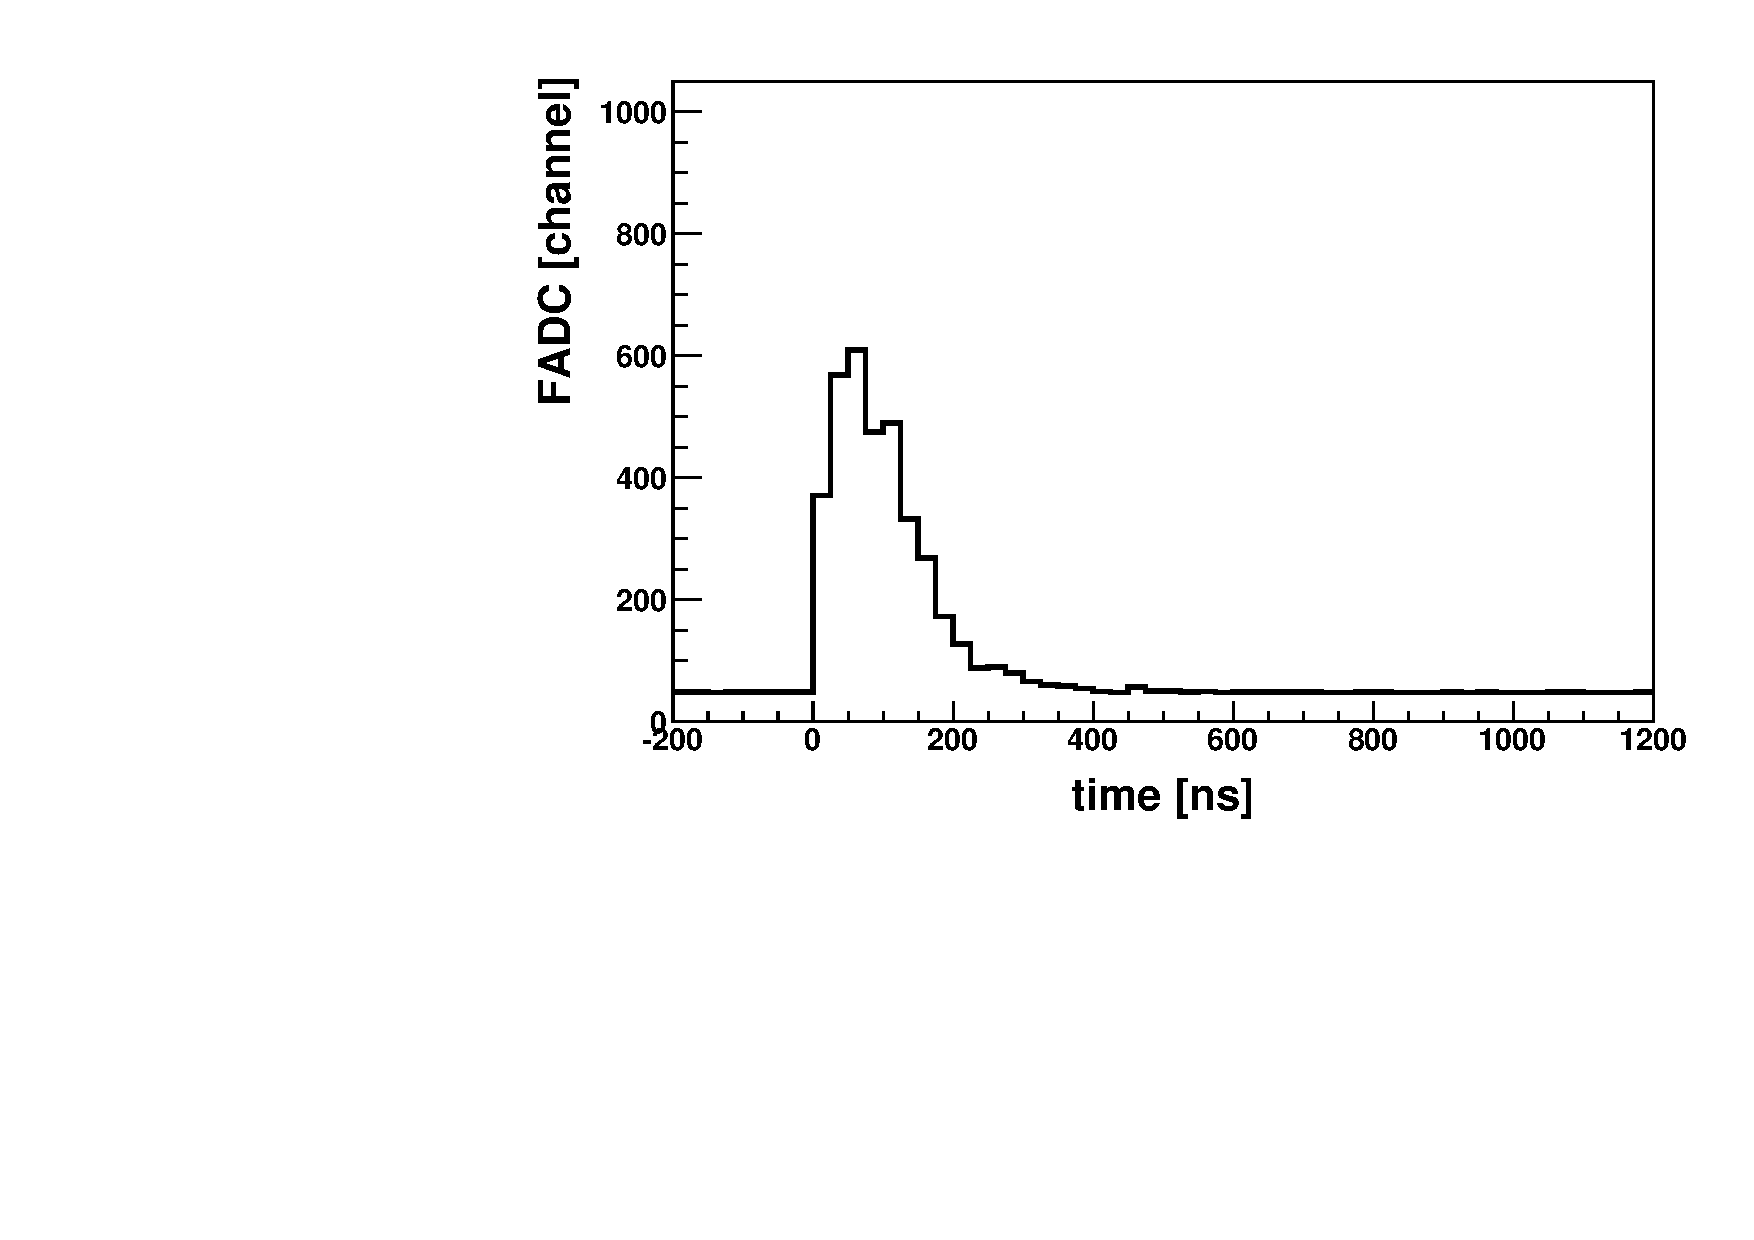
\includegraphics[width=0.47\textwidth]{fig/seleccionAuger/ev1634332_pmt1_anode.pdf} & 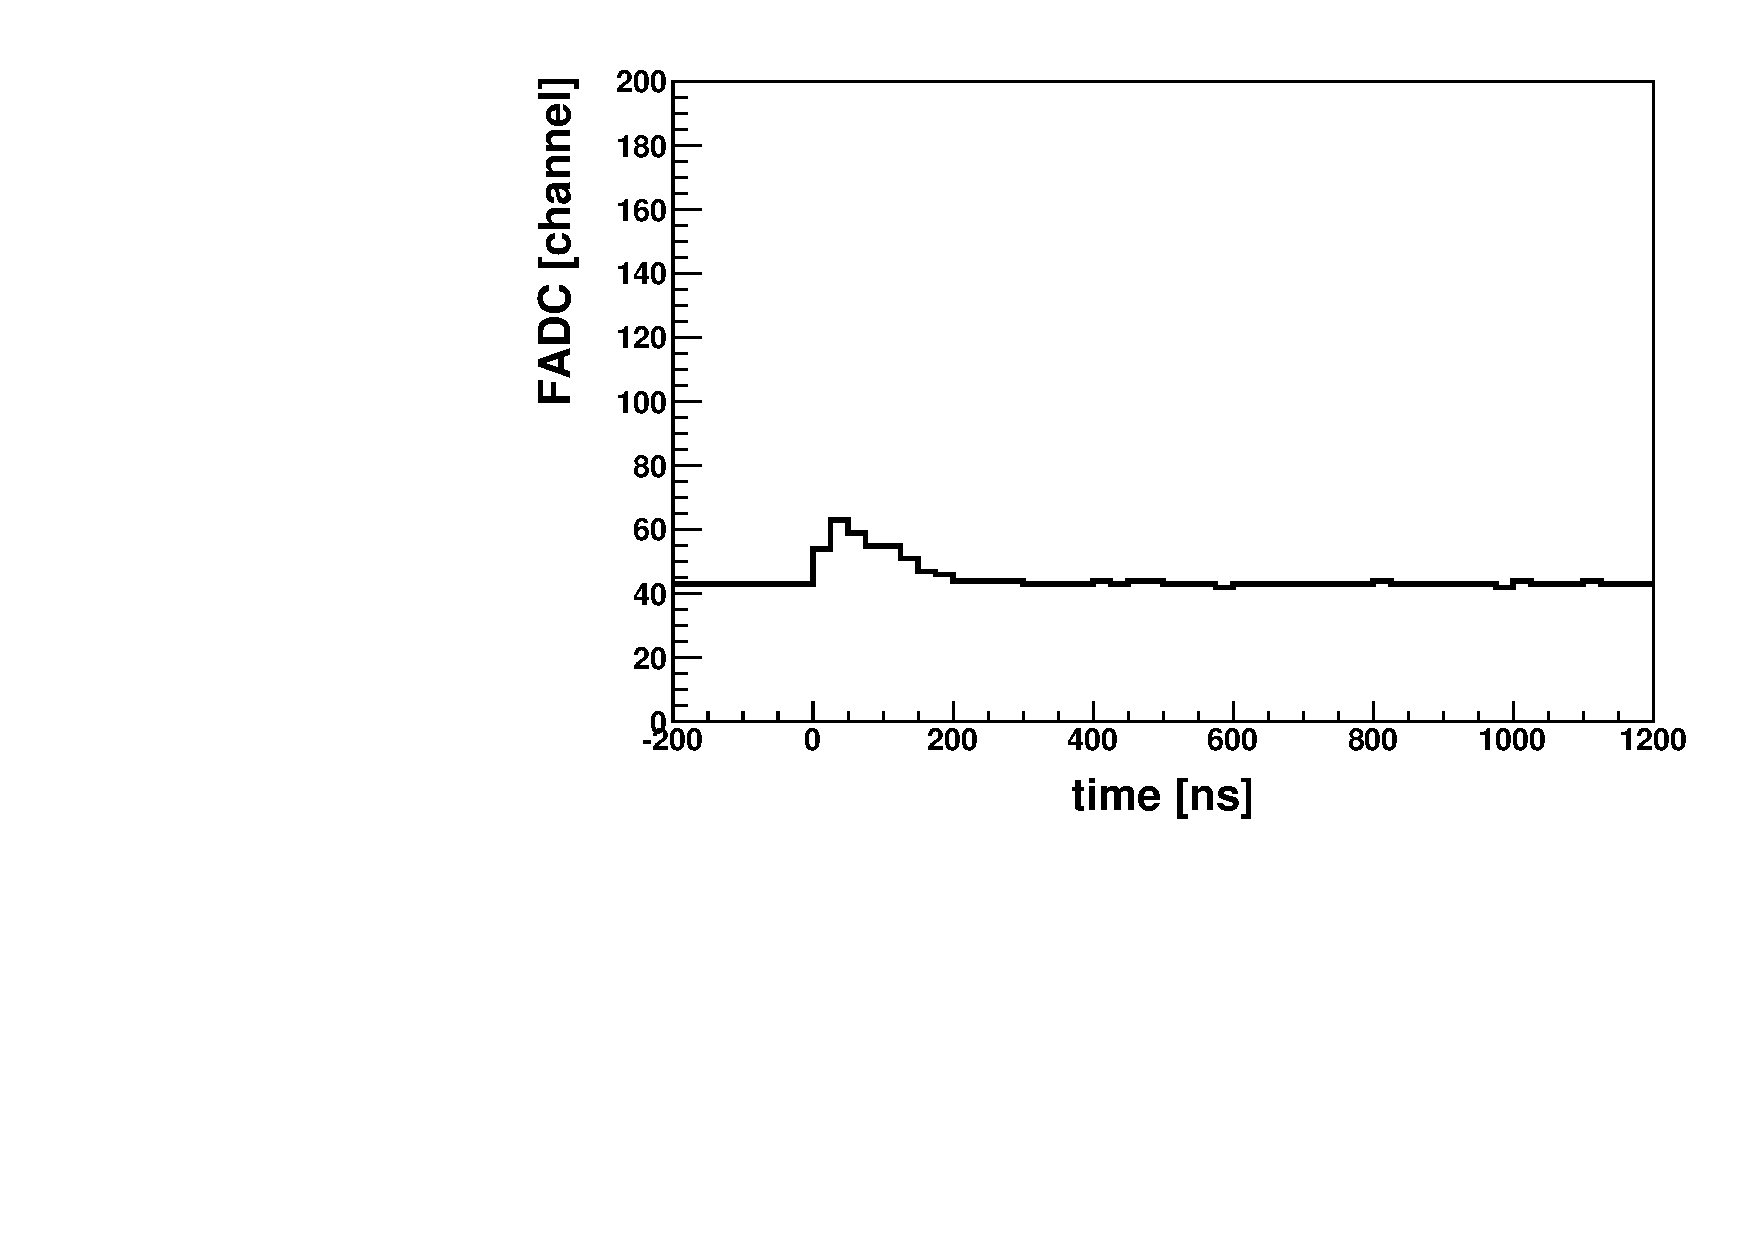
\includegraphics[width=0.47\textwidth]{fig/seleccionAuger/ev1634332_pmt1_dynode.pdf}\\
			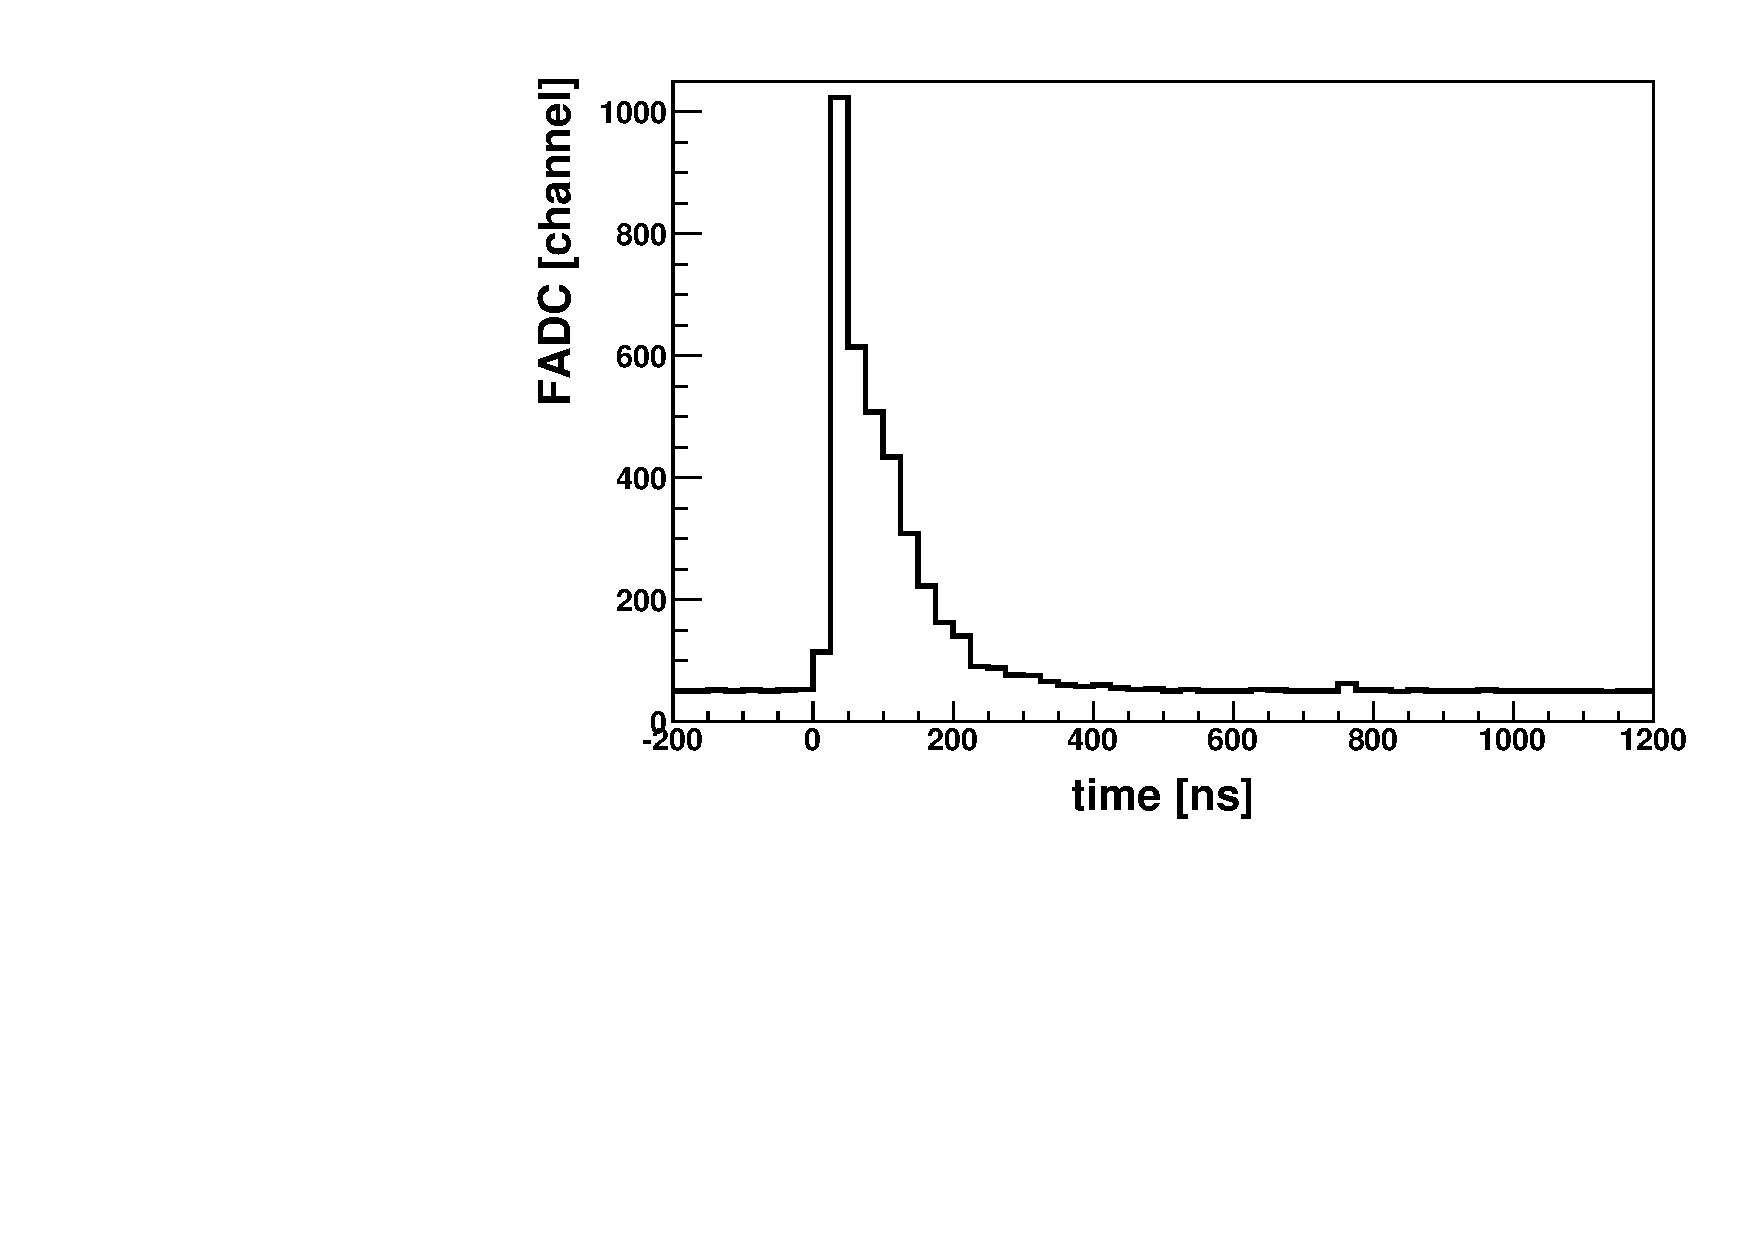
\includegraphics[width=0.47\textwidth]{fig/seleccionAuger/ev1634332_pmt2_anode.pdf} & 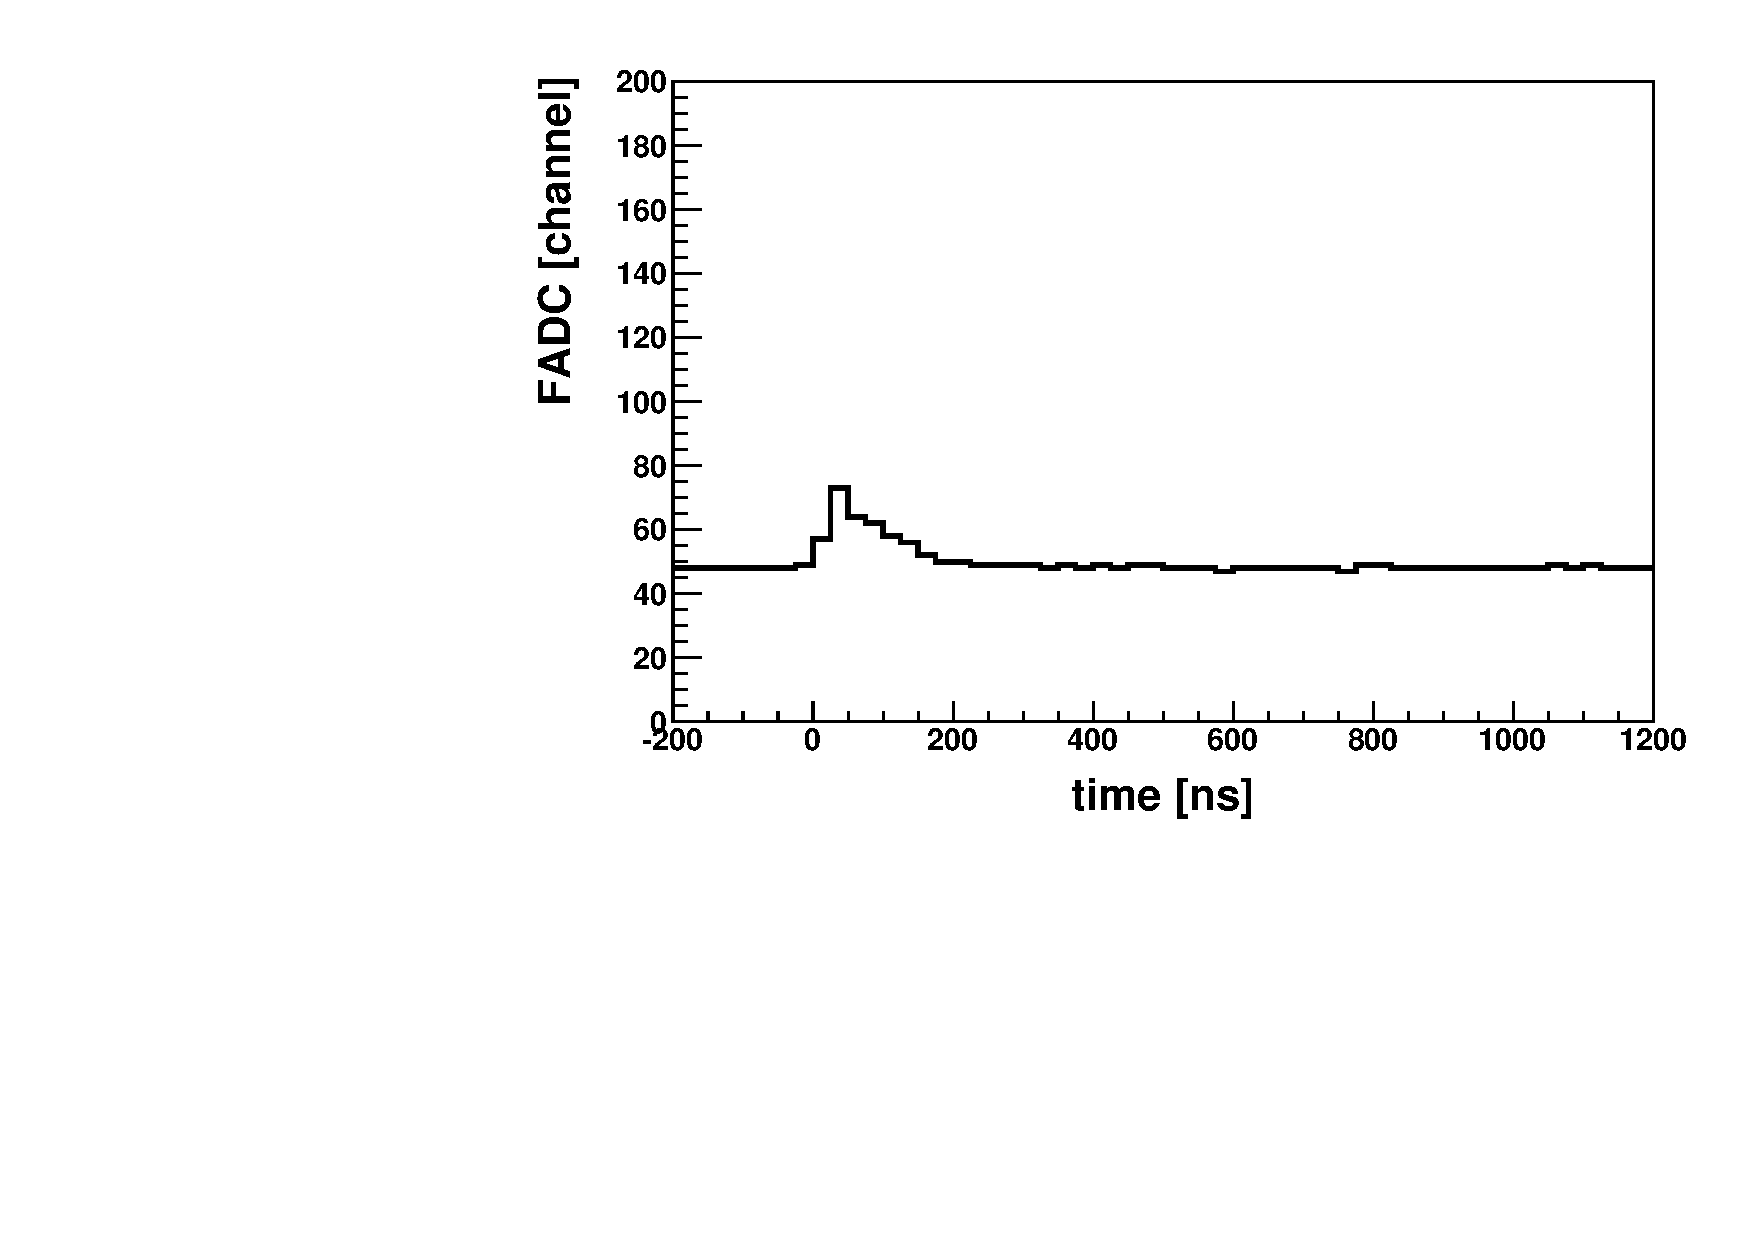
\includegraphics[width=0.47\textwidth]{fig/seleccionAuger/ev1634332_pmt2_dynode.pdf}\\
			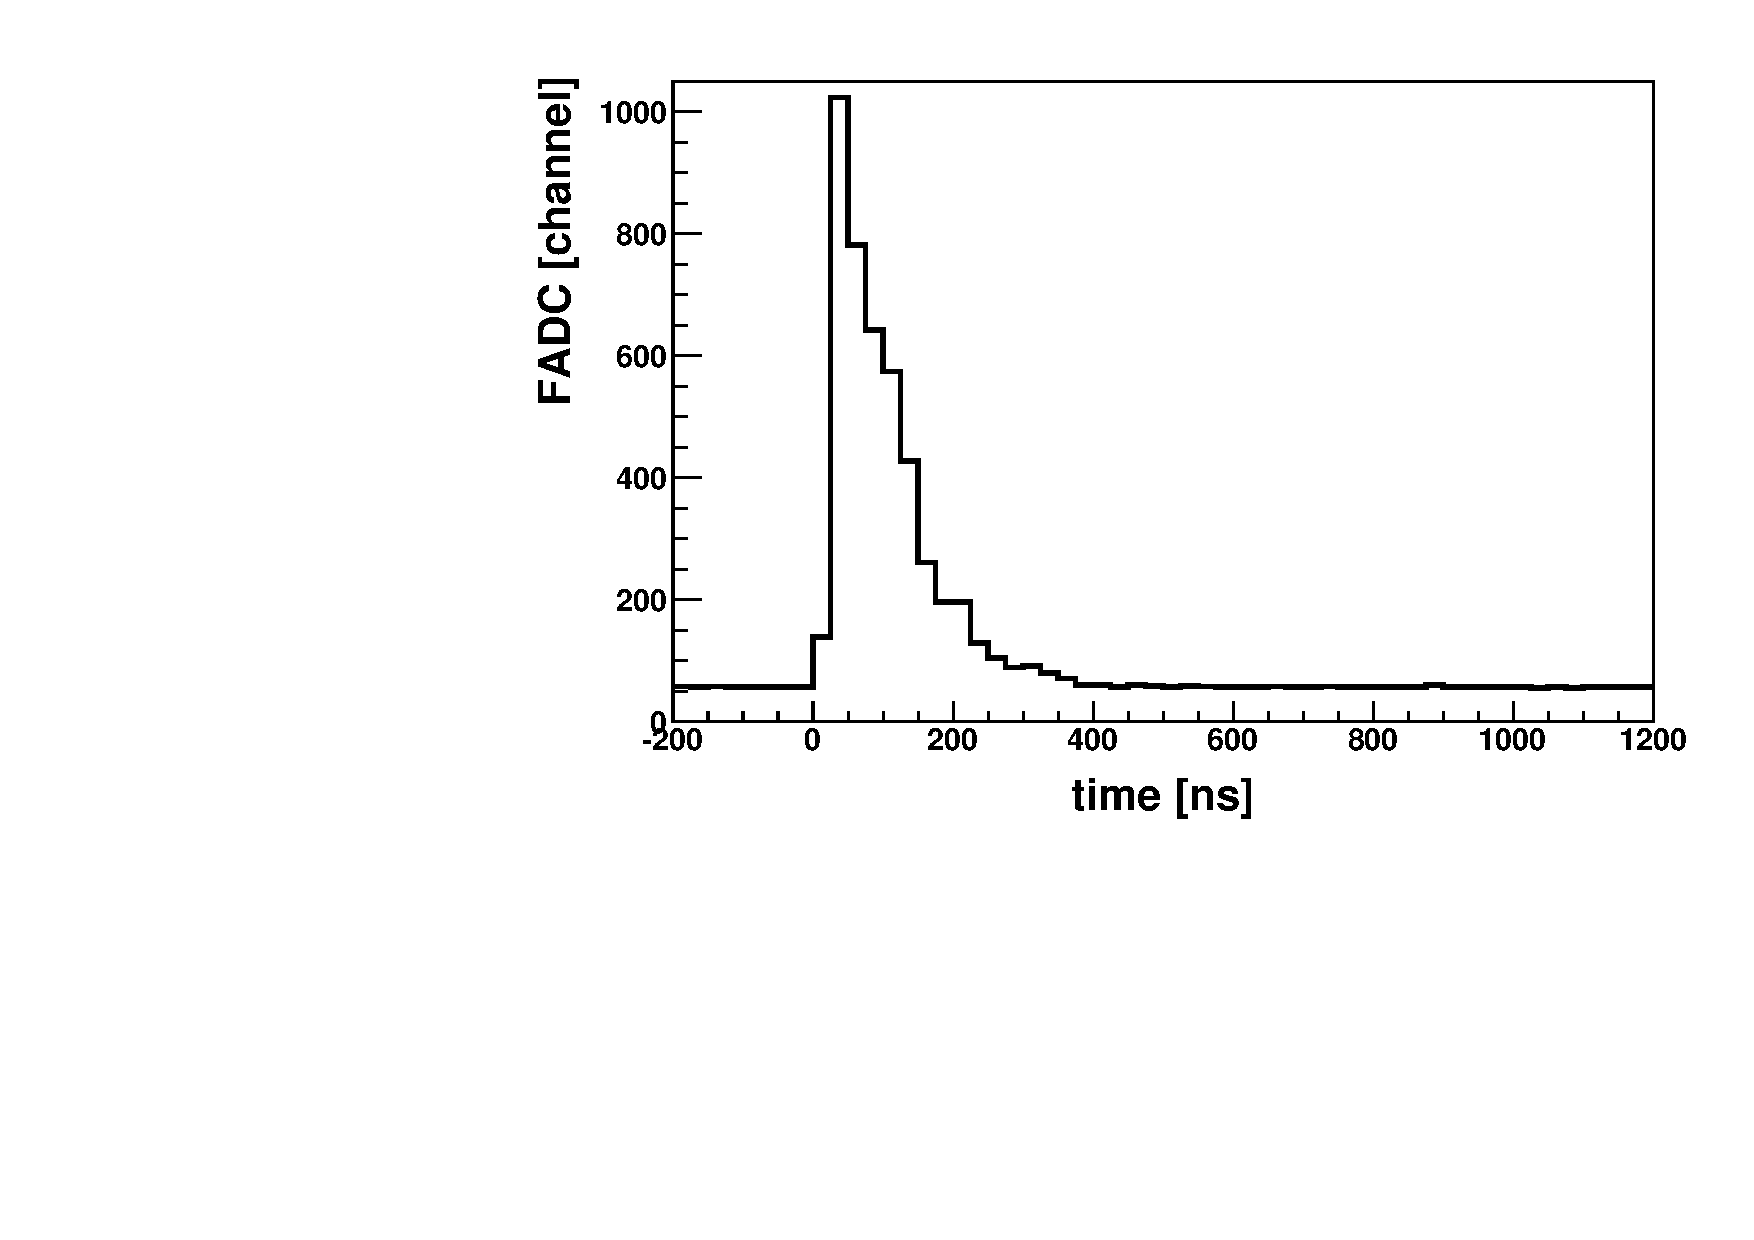
\includegraphics[width=0.47\textwidth]{fig/seleccionAuger/ev1634332_pmt3_anode.pdf} & 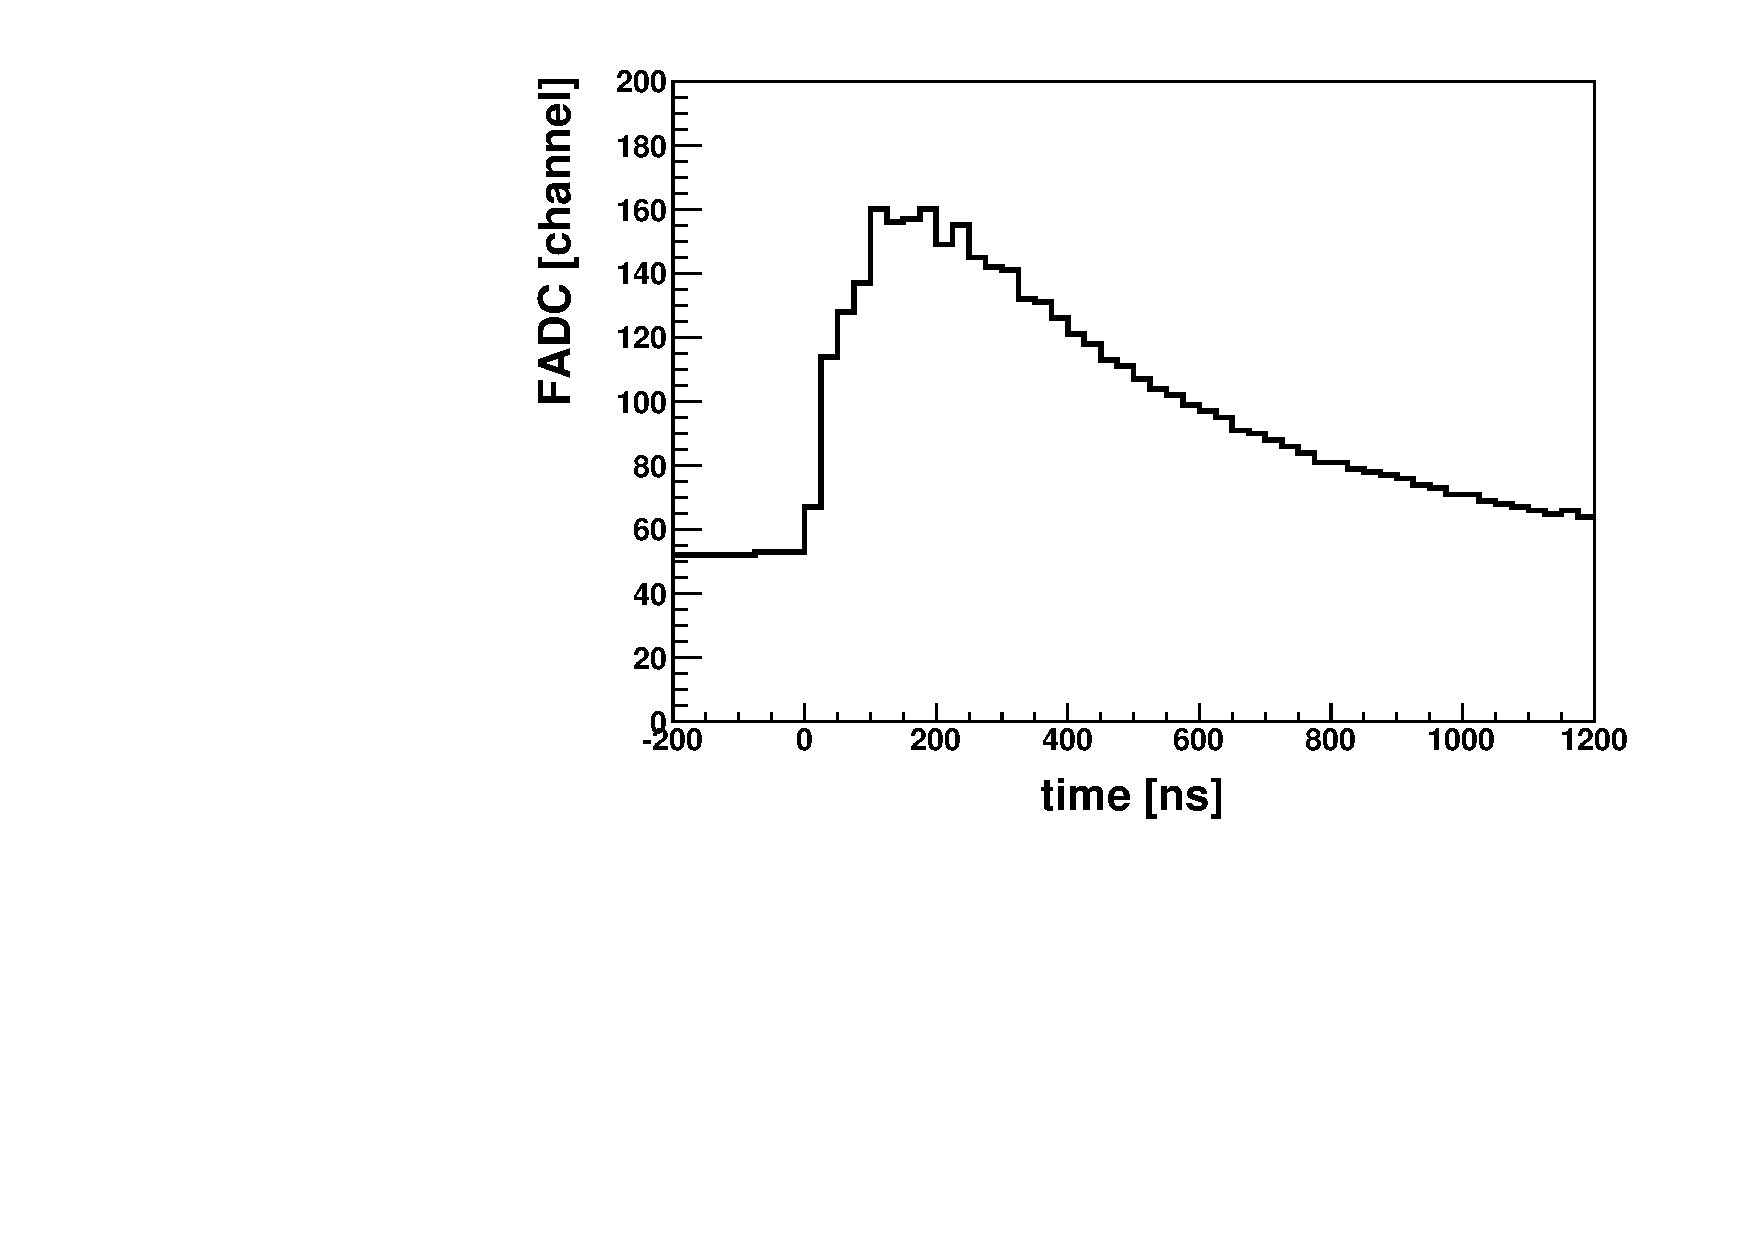
\includegraphics[width=0.47\textwidth]{fig/seleccionAuger/ev1634332_pmt3_dynode.pdf}\\
			\end{array}
			$
			\caption{Ejemplo de un PMT descartado. 
			Estación número 717 (Bobik) en el evento 1634332 detectado el 19 de Septiembre de 2005.
			De arriba hacia abajo PMT's de 1 a 3.
			En la columba izquierda (derecha) se muestra la FADC del ánodo (dínodo).
			El PMT's 3 es rechazado por tener la relación dínodo/ánodo pequeña.
			}
			\label{fig:event1634332}
			\end{center}
		\end{figure}
		
		
		\subsubsection{Criterios basados en la forma de la señal}
		
		Cuando además de la integral de la señal se presta atención a la forma de la misma, otro tipo de patologías salen a la luz, la mayoría de las veces dando lugar a un exceso de señal en la traza.
		
		Para detectar este tipo de PMT's prblemáticos se diseñó un procedimiento especial, que se detalla a continuación:
		\begin{enumerate}
		 \item Se calculan las integrales de las señales en el dínodo correspondientes a la última mitad de la traza ($\Sigma_i$, con $i$ corriendo sobre los PMT's).
		 \item Se descuenta a cada $\Sigma_i$ el bin de mayor señal y su entorno, para eliminar pulsos generados por muones accidentales.
		 \item Se etiqueta un PMT como dudoso si se cumple:
		 \begin{itemize}
		  \item La estación posee al menos dos PMT's activos.
		  \item El máximo $\Sigma_i$ es mayor a \cant{4}{VEM} y al menos 7 veces mayor que el resto.
		 \end{itemize}
		\end{enumerate}
		
		Si determinado PMT es estiquetado como dudoso durante un período de tiempo largo se lo considera un indicador de que presenta mal funcionamiento y se lo descarta.
		
		La figura \ref{fig:event3995196} muestra un ejemplo de este comportamiento. 
		
		\begin{figure}[h!]
			\begin{center}
			$
			\begin{array}{cc}
			%  \raisebox{0.8\height}{\includegraphics[width=0.4\textwidth]{fig/mapEvent1634332.png}} & 
			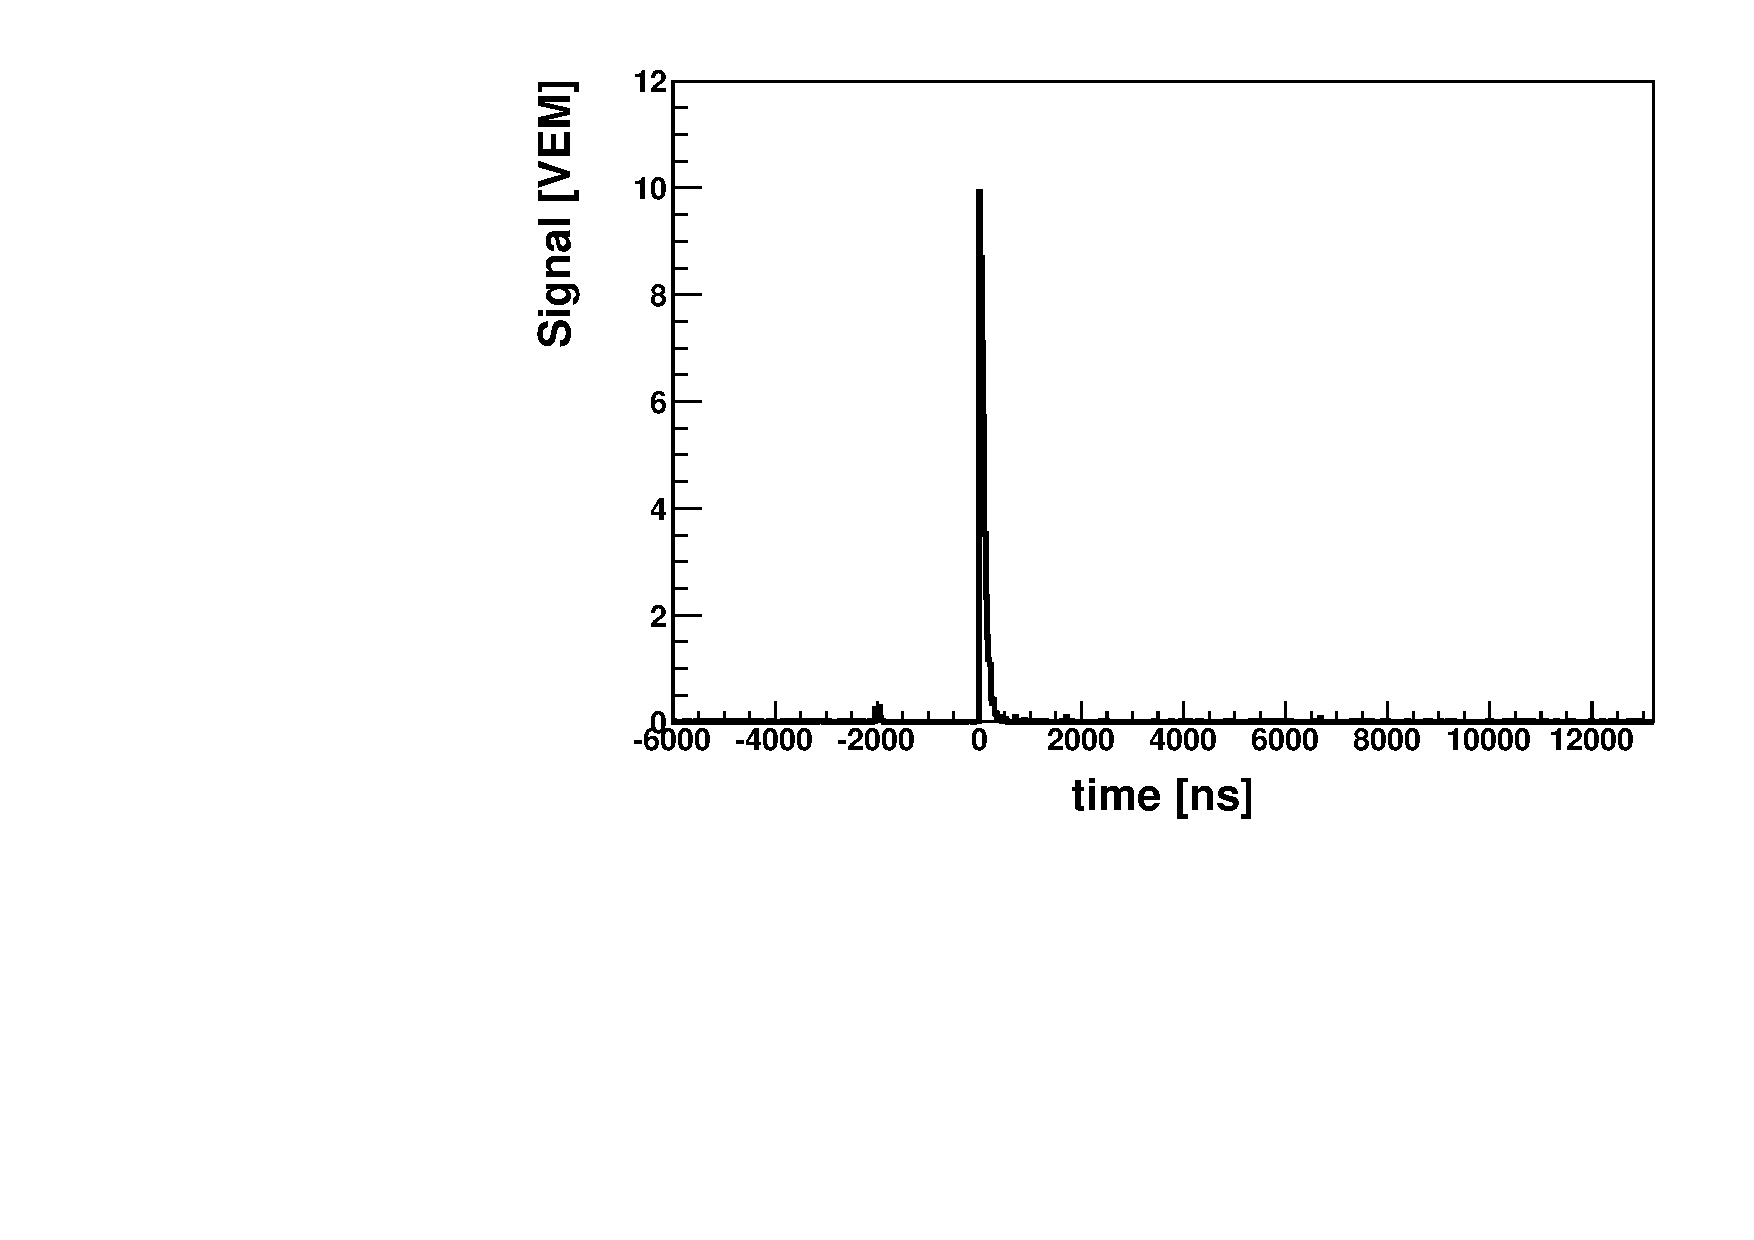
\includegraphics[width=0.6\textwidth]{fig/seleccionAuger/ev3995196_pmt1_anode.pdf}\\
			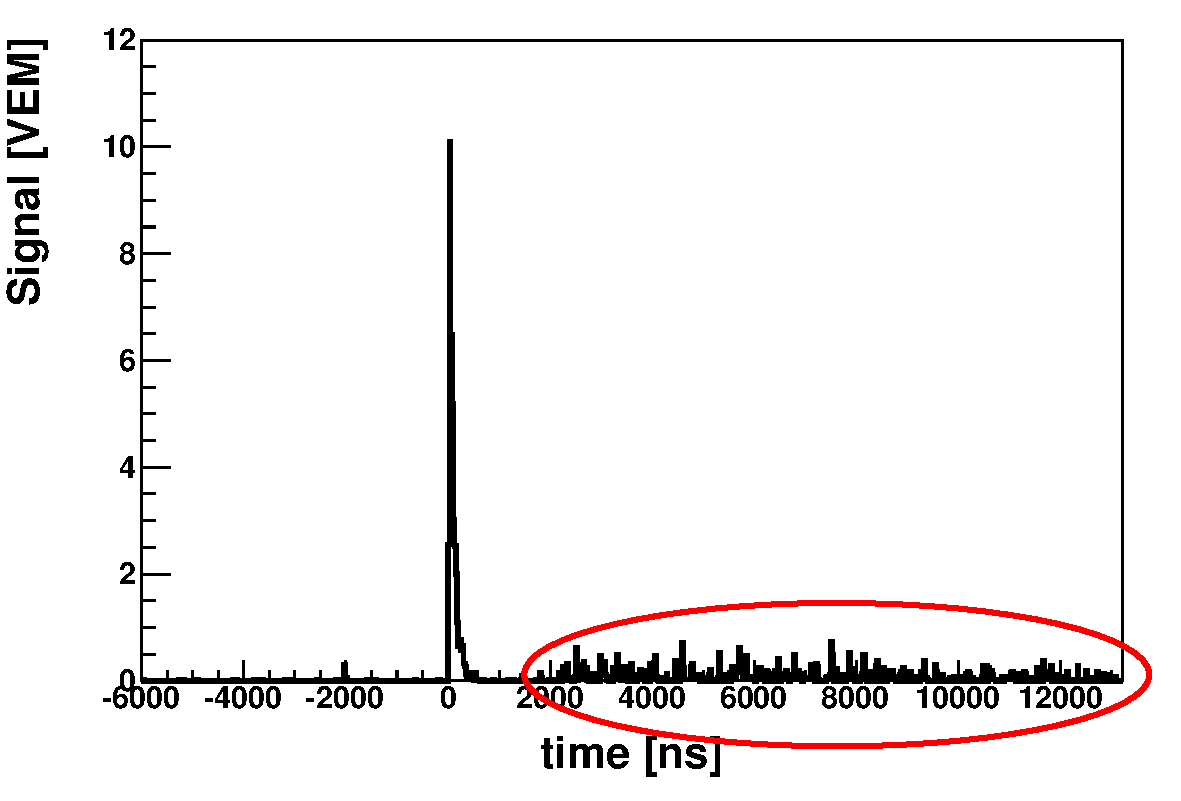
\includegraphics[width=0.6\textwidth]{fig/seleccionAuger/ev3995196_pmt2_anode_withEllipse.pdf}\\
			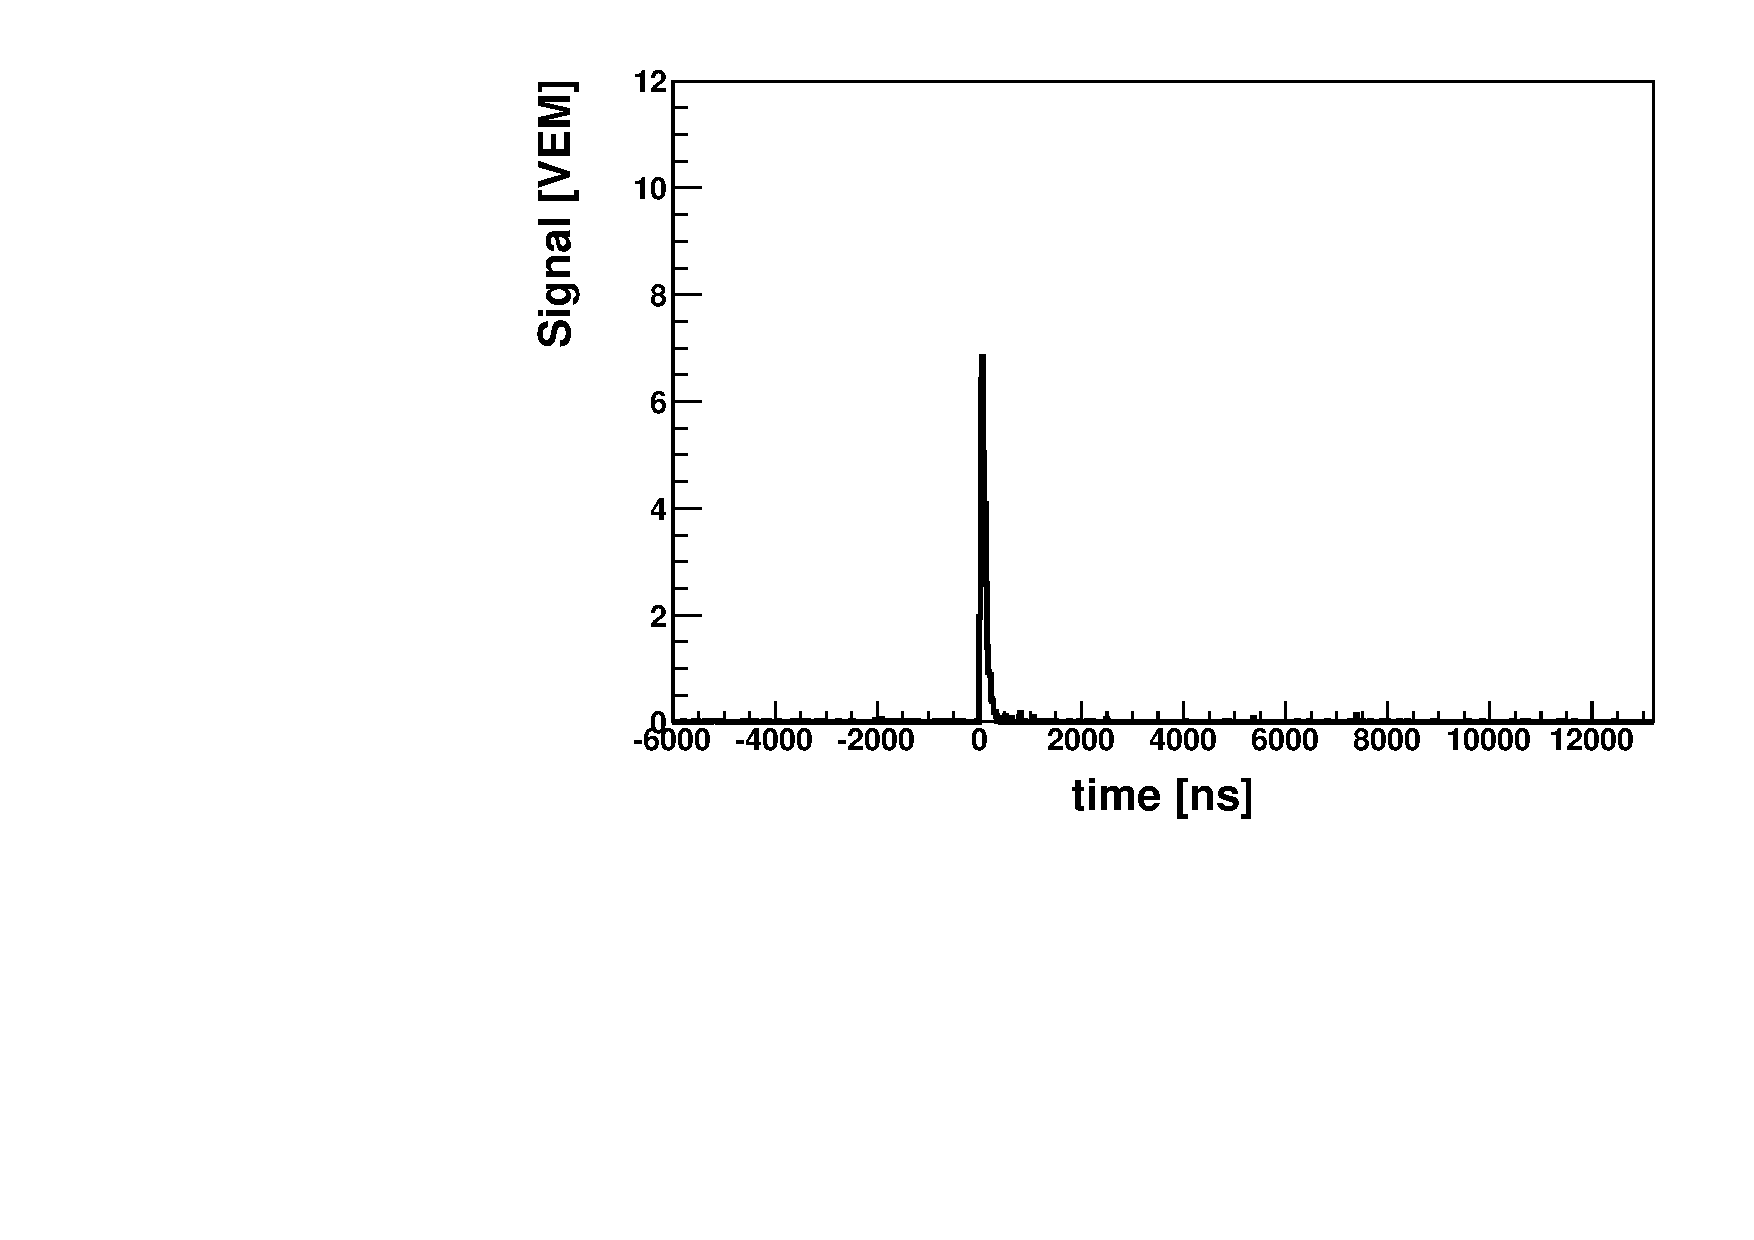
\includegraphics[width=0.6\textwidth]{fig/seleccionAuger/ev3995196_pmt3_anode.pdf}
			\end{array}
			$
			\vspace{-0.5cm}
			\caption{
			Ejemplo de un PMT descartado por permanecer como dudoso por un período largo de tiempo.
			Estación 1440 (Nirvana) para el evento 3995196 con fecha 28 de Septiembre de 2007.
			De arriba a abajo, PMT 1 a 3. El PMT número 2 se estiqueta como dudoso. La etiqueta se debe a la señal espúrea que se señala con una elípse sobre el final de la traza.
			}
			\label{fig:event3995196}
			\end{center}
		\end{figure}

	\subsection{Seleccion de estaciones}
	
	Hay varias rasones para descartar estaciones. Por ejemplo algunas de ellas poseen un solo PMT activo durante algún período de tiempo, o si cierto evento fue registrado durante una tormenta eléctrica, puede ser que la señal de radio emitida por un relámpago haya interferido con la electrónica, o simplemente algúm muon accidental disparó la estación que realmente no forma parte del evento.
	A continuación se detallan los procedimientos para descartar este tipo de anomalias.
	
		\subsubsection{Estaciones con un solo PMT activo}
		
		Aunque cada estación cuenta con 3 PMT's algunos pueden tener fallas temporales o permanentes, lo que hace necesario eliminarlos del análisis.
		Dado que la superficie instrumentada es inmensa e incluso a veces de dificil acceso, reemplazar o arreglar un PMT que presenta fallas puede llevar meses.
		Si un candidato a neutrinos apareciera, es necesario poder confirmar la señal en la estación por con al menos dos PTM's. 
		Si bien es raro, es posible que suceda que una estación siga funcionando con un PMT activo.
		En este caso, no sería posible realizar la confirmación de la traza, por lo que esa estación se descartaría del evento.
		
		\subsubsection{Estación con señales debidas a relámpagos}
		
		Una posible fuente de señales espúreas son los relámpagos.
		Cuando la señal electromagnética que generan alcanza la electrónica de adquisición de las estaciones, se registra una señal oscilante en el orden de los $\rm MHz$, como se observa en la figura \ref{fig:event1186354_st506_pmt}.
		%
		\begin{figure}[th!]
		\begin{center}
		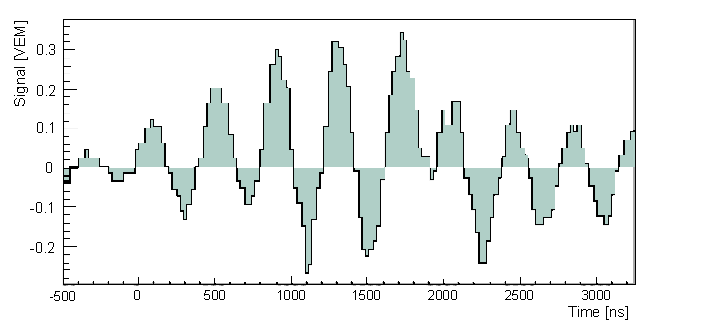
\includegraphics[width=0.7\textwidth]{fig/seleccionAuger/event3995197_station506_pmt3.pdf}
		\caption{Ejemplo de una señal generada por un relámpago.
		La señal corresponde al PMT número 3 del evento 3995197 con fecha 26 de enero de 2005.}
		\label{fig:event1186354_st506_pmt3}
		\end{center}
		\end{figure}
		% 
		La oscilación en la señal se usa para detectar este tipo de sucesos.
		Si un evento contiene una estación de este tipo, se descarta.
		
		\subsubsection{Estaciones accidentales: efecto de los muones atmosféricos}
		
		El detector se encuentra expuesto a un flujo constante de muones atmosféricos mucho mas abundante que el de UHECR\footnote{Estos incluso se utilizan para el calibrado automático de las estaciones.}. 
		Al nivel del detector, \cant{1400}{m} sobre el nivel del mar, este se compone principalmente de muones en el rango de \cant{1-10}{GeV}. 
		Estas partículas, que no forman parte de los eventos que nos interesan, pueden afectar la reconstrucción de dos maneras:
		%
		\begin{enumerate}
		\item \textbf{Producir un trigger T2 en una estación de superficie que no pertenece al evento:} como las partículas que disparan la estación no pertenecen a la lluvia, el tiempo del T2 adicional tendrá una distribución uniforme en la ventana de 60~$\mu$seg del T3. Como la selección de lluvias inclinadas depende fuertemente de las posiciones y tiempos de disparo de las estaciones, una estación extra puede dar como resultado una incorrecta estimación de la geometría de la lluvia, especialmente en los eventos más pequeños.

		\item \textbf{Agregar señal espuria en alguna de las estaciones que sí pertenecen al evento:} si la señal accidental ocurre unos pocos $\mu$seg antes de que las partículas de la cascada atmosférica alcancen la estación, el resultado es que ambas señales se fusionan en una misma traza, siendo la señal espuria la que fija el tiempo de disparo del T2 producido (ver figura \ref{fig:trazaMalTiempo}). Esta modificación en el tiempo de disparo tiene efectos sobre la reconstrucción del evento. 
		Además del posible efecto sobre el tiempo de disparo, la señal espuria modifica los valores de los observables de la traza incluso si arriba unos $\mu$seg despúes que las partículas de la cascada. Como se discutirá más adelante, este efecto puede ser importante y será tenido en cuenta en la elaboración del criterio de identificación de neutrinos. 
		\end{enumerate}
		%
		\begin{figure}[ht]
		\begin{center}
		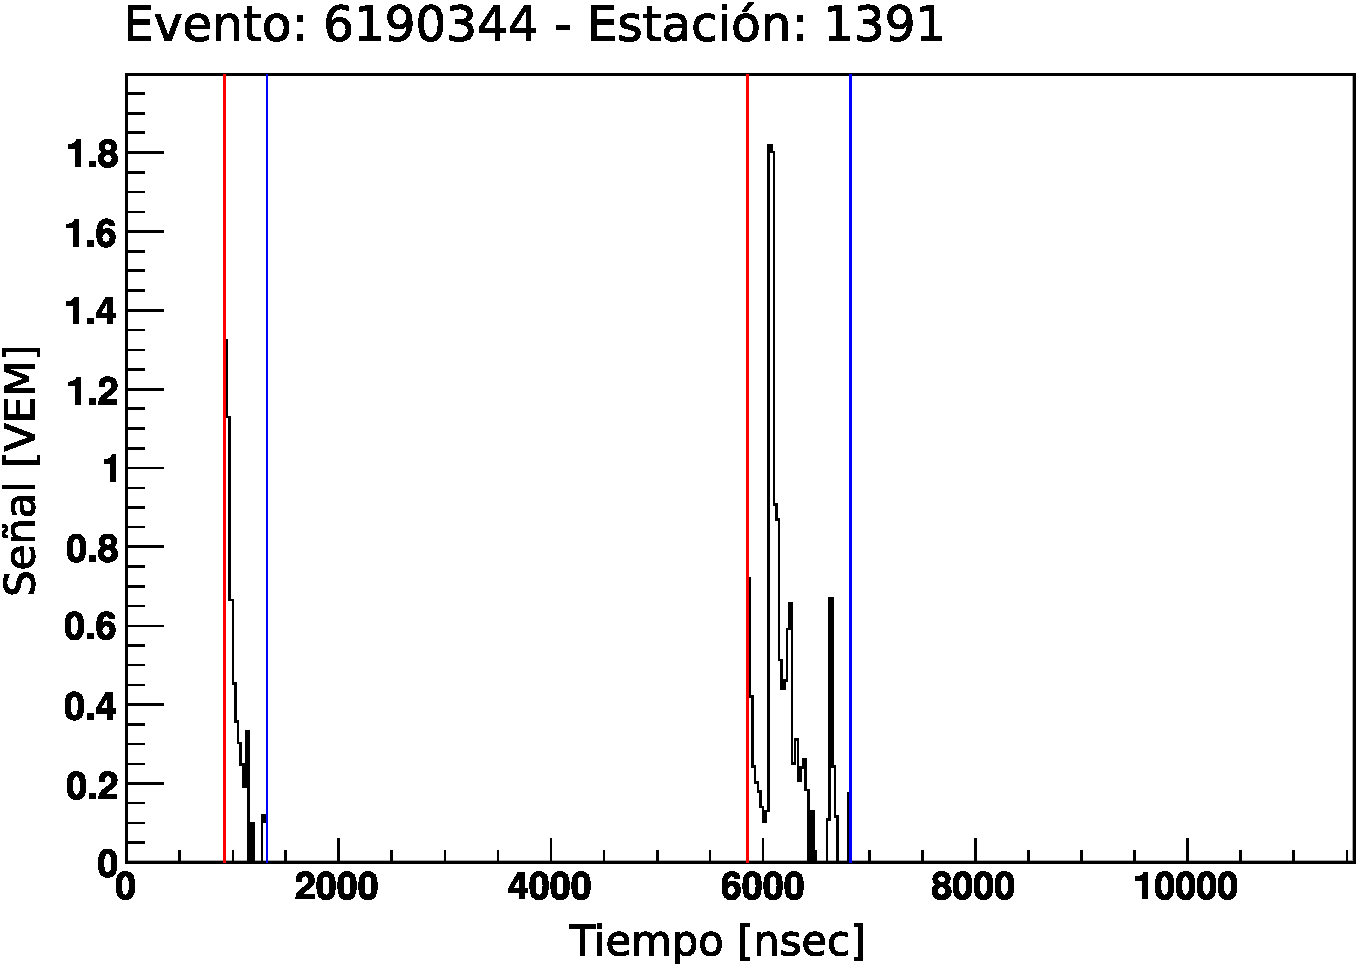
\includegraphics[width=0.75\textwidth]{fig/seleccionAuger/badStartTime.pdf}
		\caption{Efecto de un muón accidental en la determinación errónea del tiempo de disparo.}
		\label{fig:trazaMalTiempo}
		\end{center}
		\end{figure}
		
		Con el fin de minimizar el impacto de estas señales espúreas que producen los muones accidentales se aplica el siguiente procedimiento.
		
		\titulo{Algoritmo de limpieza de traza} la idea del método es simple, la cantidad de energía que los muones depositan en el tanque es, a primer orden, proporcional a la longitud del camino que recorren dentro del tanque.
		Dado que las estaciones son bastante más anchas que altas (\cant{1.2}{m} de alto por \cant{3.6}{m} de diametro), los muones inclinados producen una señal que, en promedio, es mayor que la producida por los verticales.
		
		Los muones accidentales son mayormente verticales como se puede ver figura \ref{fig:atmo_mu_flux}.
		Este hecho puede ser explotado para identificar qué fracción de la traza debe ser eliminada.
		%
		\begin{figure}[ht]
		\begin{center}
		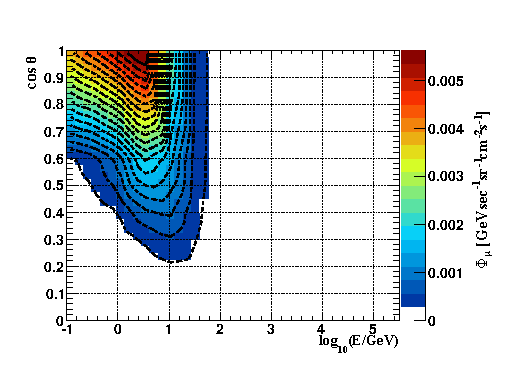
\includegraphics[width=0.85\textwidth]{fig/seleccionAuger/atmo_mu_flux.pdf}
		\caption{Flujo de muones atmosféricos de acuerdo con la parametrización dada en~\cite{cite:atmo_mu}. Puede observarse que la mayoría presenta un ángulo cenital inferior a 50$^{\circ}$ ($\cos\theta \geqslant 0.6$)}.
		\label{fig:atmo_mu_flux}
		\end{center}
		\end{figure}
		
		El algoritmo de limpieza utilizado se describe en \cite{trace_cleaning}.
		Este comienza al nivel de cada PMT dentro del tanque:
		%
		\begin{enumerate}
		 \item Se extraen los segmentos de señal de cada PMT, definidos por al menos 2 bines consecutivos que presenten al menos 3 unidades de FADC por sobre la linea de base.
		 Se guardan los índices de inicio y fin, y se calcula la carga de cada segmento $Q$ y su pico $P$.
		 \item Se unen los segmentos si el gap entre ellos es de menos de 20 bines mas la longitud del primer segmento, y si al menso una de las siguientes condiciones se cumplen:
		 \begin{enumerate}
		  \item El primer segmento posee una señal $Q_1>0.3Q_2$
		  \item El segundo segmento posee de menos de 5 unidades FADC sobre la linea de base
		 \end{enumerate}
		El objetivo de estas condiciones es unir segmentos que hayan sido provocados por partículas de la lluvia.
		\item Se combinan las señales de los diferentes PMT's, combinando los segmentos que se superpongan mediante el promedio.
		\item El start time de los segmentos combinandos se toma de la contribución que posea la mayor señal.
		\end{enumerate}
		
		Como ejemplo, en la figure \ref{fig:atmo_mu_flux}, el algoritmo encuentra dos segmentos.
		En principio, el segmento con la señal integrada mas grande se conserva y el resto se descarta.
		Sin embargo, tambien podría ocurrir que uno o mas segmentos posean una señal similar, por lo que no sería claro cuál es el segmento que realmente interesa.
		Para salvar estas situaciones, se aplica un algoritmo especial, comenzando por segmentar la señal promedio con un criterio similar al que se aplica para segmentar la de los PMT's:
		%
		\begin{enumerate}
		 \item El segmento comienza con el primer bin que presente una señal por encima de los \cant{0.2}{VEM}.
		 \item En los siguientes 10 bines (\cant{250}{ns}) la carga integrada $Q$ debe superar los \cant{3}{VEM}. Si no, el inicio de la traza se muebe un bin hacia adelante hasta que las ambas condiciones se cumplan.
		 \item El final de la señal se define cuando a partir de él se encuentren 15 bines consecutivos por debajo de \cant{0.2}{VEM}.
		 \item Se calculan dos cantidades:
		 \begin{enumerate}
		  \item $nBoT$: el numero de bines por encima de \cant{0.2}{VEM}.
		  \item $Q_T$: la suma de la señal sobre los bines sobre \cant{0.2}{VEM}.
		 \end{enumerate}
		\end{enumerate}
		%
		A cada segmento se le asigna una puntuación $s=nBoT\times Q_T$. 
		Las trazas inducidas por muones atmosféricos tienden a tener valores de $s$ pequeños cuando se los compara con las inducidas por lluvias inclinadas.
		Si hubiera más de un segmento que cumpla $s>0.5s_{max}$, con $s_{max}$ la máxima puntuación, la estación es rechazada debido a que el tiempo de inicio de la señal es ambiguo.
		En caso contrario, el segmento con mayor puntuación se conserva y el resto se rechaza.
		La figura \ref{fig:multipicos} muestra un ejemplo de una estación que muestra tres segmentos similares. 
		%
		\begin{figure}[ht]
			\begin{center}
			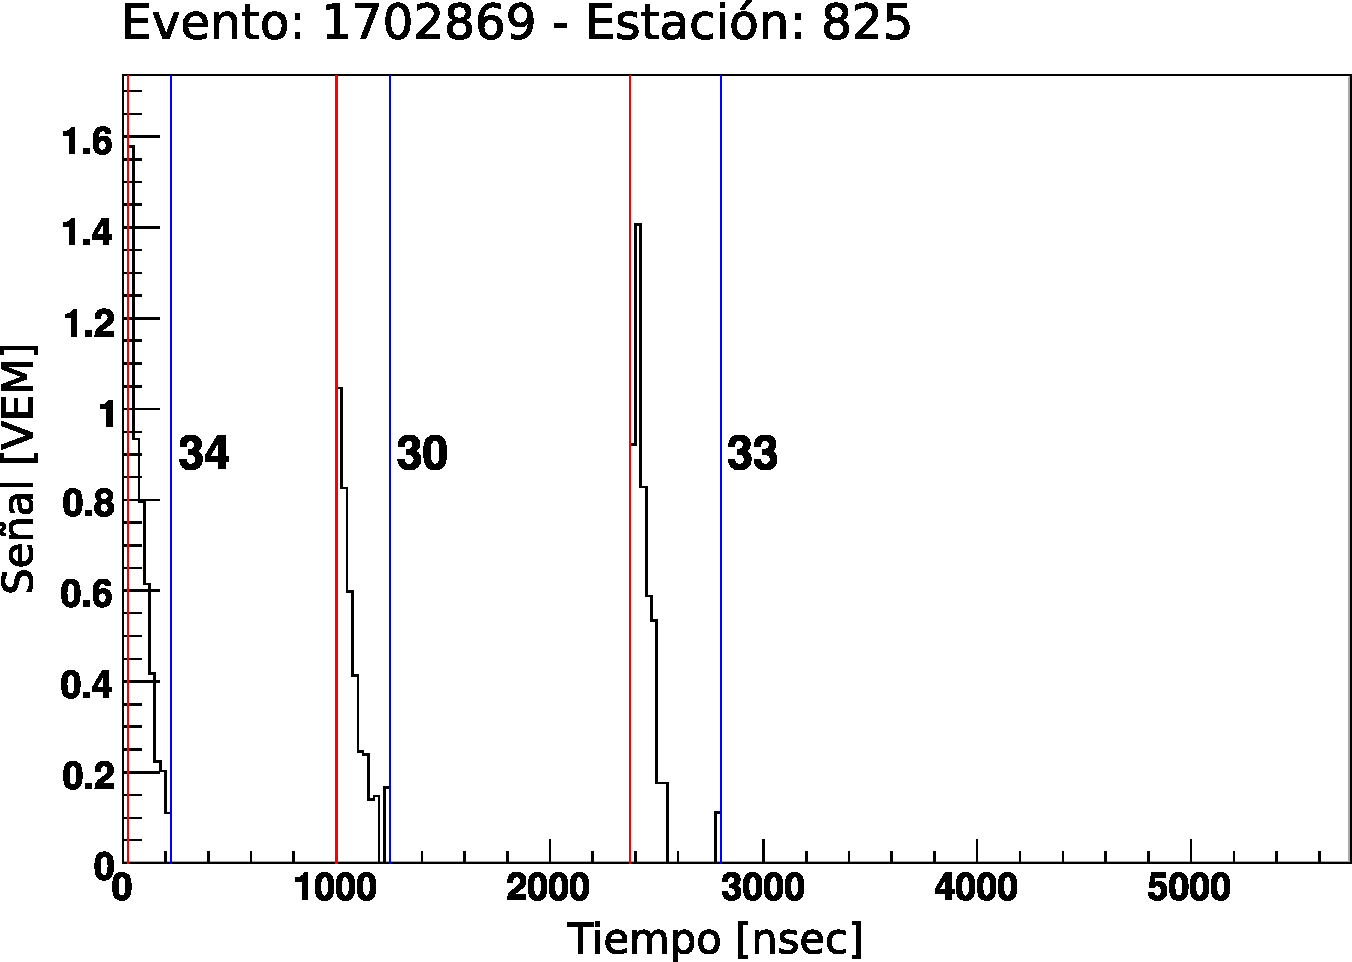
\includegraphics[width=0.75\textwidth]{fig/seleccionAuger/multipicos.pdf}
			\caption{Traza que presenta múltiples segmentos de señal con características similares en la que no es posible determinar el tiempo de disparo T2. Los valores resaltados indican el puntaje asignado a cada segmento.}
			\label{fig:multipicos}
			\end{center}
		\end{figure}
		%
		Esta estación es removida del evento antes de aplicarle la reconstrucción.
		
	\subsection{Reconstrucción preeliminar}
	
	Una vez aplicados los precedimientos descriptos hasta el momento, los eventos cuentan con una lista de escaciones cuyos tiempos de disparo T2 se encuentran bien definidos.
	Sin embargo, los evetos todavia pueden contener estaciones disparadas por muones atmosféricos o incluso por una lluvias de baja energía.
	Con el fin de identificar las estaciones que realmente pertenecen al evento que nos interesa, se pide que las estaciones pertenecientes a los eventos satisfagan una serie de requerimentos de compacticidad espacial y temporal.
	
	\subsubsection{Eliminación de estaciones aisladas} 
	
	El primer paso es remover las estaciones aisladas pidiendo las siguientes dos condiciones:
	\begin{enumerate}
	 \item Criterio estandar: Se elimina una estación como aislada si no cuple que:
	 \begin{enumerate}
	  \item Existe una estación con T2 a menos de tres coronas, \cant{d_1=4700}{m}, y dentro de un rango temporal de compatible con un frente que se desplaza a la velocidad de la luz, \cant{t_1=\frac{d_1}{c}\sim15700}{ns}.
	  \item Eciste una segunda estación con T2 en la cuarta corona, \cant{d_1=6200}{m}, y con el mismo criterio temporal, \cant{t_2=\frac{d_2}{c}\sim20700}{ns}.
	 \end{enumerate}
	 \item Eliminación de señales muónicas: Si la magnitud de la traza es compatible con la señal de un muon vertical, ${\rm AoP} \equiv \frac{S}{S_{peak}}<1.4$, el criterio es mas estricto, pidiendo al menos una señal con T2 en la primer corona o en las estaciones cercanas de la segunda, \cant{d=2700}{m}.
	\end{enumerate}
	
	\subsubsection{Selección Top-Down} 
	
	El segundo paso consiste en la selección de estaciones compatibles con haber sido disparadas por el frente de partículas de una EAS.
	El algoritmo utilizado para este propósito se conoce como \emph{selección Top-Down} \cite{topDownSel}.
	
	La idea general del método consiste en ir descartando estaciones hasta encontrar una configuración que cumpla las condiciones requeridas.
	A continuación se expone el paso a paso del algorítmo:
	%
	\begin{enumerate}
	 \item Se realiza una reconstrucción del ángulo cenital del evento $\theta_{rec}$ asumiendo un frente plano y un tiempo de arrivo $t_0$, definido como el tiempo promedio de inicio de señales y pesado por las mimas. Este procedimiento se realiza analiticamente como se detalla en el apéndice \ref{ap:topDown}
	 \item Se evalua la compatibilidad temporal para cada estación y para el evento completo evaluando:
	 \begin{itemize}
	  \item $\Delta t_i < (N-2)\cdot 250{\rm ns} \cdot {\rm max}(\cos\theta_{rec},0.2)$
	  \item $\sum_i\Delta t_i^2 < \left[(N-2)\cdot 200{\rm ns} \cdot {\rm max}(\cos\theta_{rec},0.2)\right]^2$
	 \end{itemize}
	 donde $\Delta t_i$ es la diferencia entre el tiempo de T2 de la estacion $i$ y el obtenido mediante el ajuste del frente plano.
	 
	 Los cortes dependen de la multiplicidad del evento $N$ y de el ángulo reconstruido $\theta_{rec}$.
	 Debido a la curvatura del frente de la lluvia, las estaciones perisféricas presentan una mayor diferencia temporal respecto del frente plano que las centrales (ver figura \ref{fig:planeFrontAprox}). 
	 
	 La dependencia con el ángulo cenital aparece por una razón similar: las lluvias inclinadas llegan al detector tras atravesar mayor cantidad de materia que las verticales. Por este motivo, la dependencia del radio del frente de la lluvia se considera típicamente $R\propto\sec\theta$ \cite{cite:ShowerFront}, $R$ el radio de curvatura.
	 Consecuentemente, par ángulos cenitales grandes el frente de la lluvia presenta una curvatura pequeña ($R$ grande).
	 Para $\cos\theta < 0.2$, lo que corresponde a $\theta>80^\circ$, se asume que el mismo ha alcanzado su curvatura mínima.
	 Por esta razon, el mínimo tiempo de tolerancia para las estaciones respecto del frente plano será \cant{(N-2)50}{ns}.
	 \item Tambien se pide compacticidad espacial.
	 Todas las estaciones, proyectadas sobre el plano del frente de la lluvia, deben estar contenidas dentro de un círculo de radio $r_{max}$, con:
	 \begin{equation}
	  r_{max} = \sqrt{1300^2(N-2)}{\rm m}
	 \end{equation}
	 \item Se verifica la condición de T3.
	\end{enumerate}
	%
	\begin{figure}[ht]
	\begin{center}
	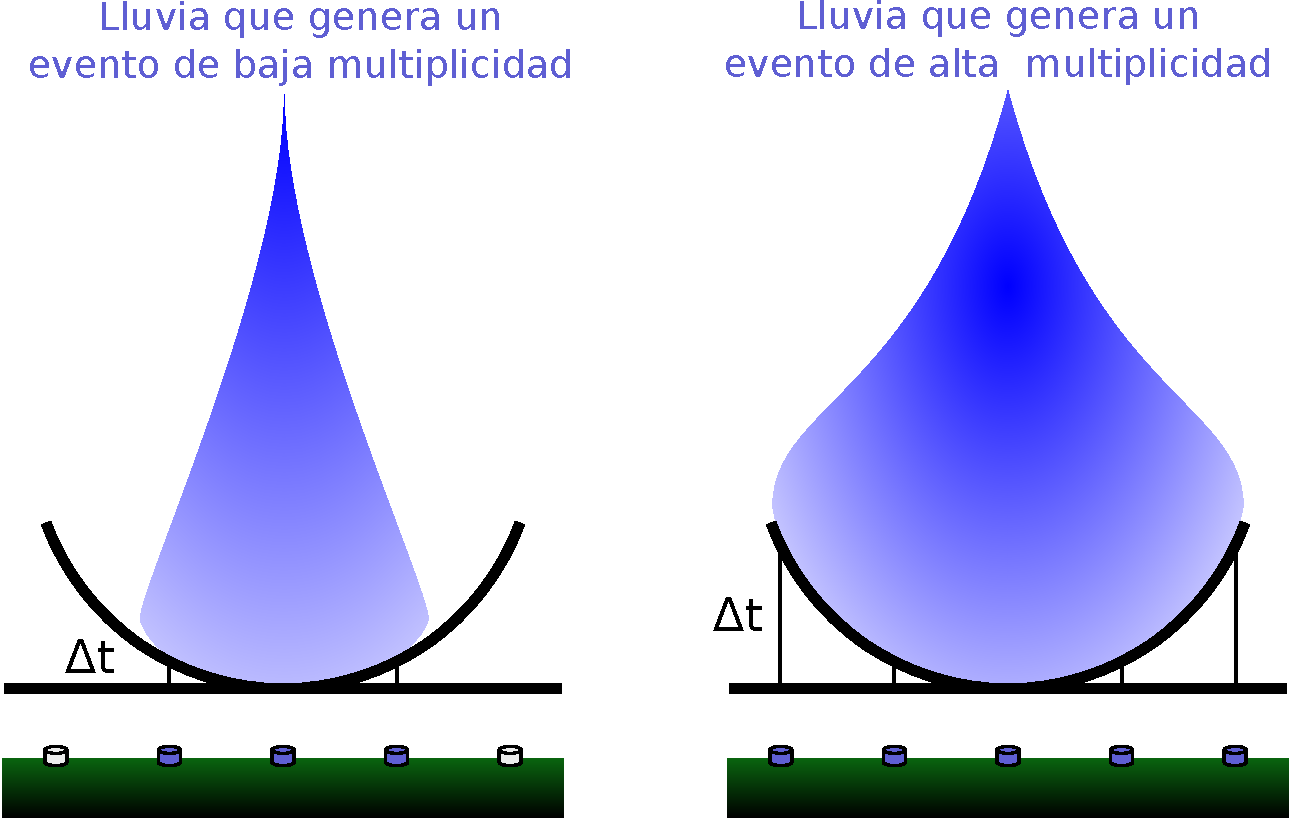
\includegraphics[width=0.85\textwidth]{fig/seleccionAuger/plano_vs_curvo.pdf}
	\caption{Esquema de la diferencia de tiempo entre un frente de lluvia curvo y su aproximación plana. 
	Las lluvias que generan alta multiplicidad de estaciones tienden a presentar diferencias de tiempo mayores al compararlas con la aproximación de frente plano.}
	\label{fig:planeFrontAprox}
	\end{center}
	\end{figure}
	%
	Si alguna de las condiciones no se satisface se intenta con las configuraciones de $N-1$ estaciones, quitando primero las de menor señal. 
	En cuanto todos los criterios se satisface, se acepta la configuración. Si no sucede, se quitan de a 2, 3 o hasta 4 estaciones.
	Si luego de probar todas las configuraciones quitando hasta 4 estaciones no se encontró ninguna configuración que satisfaga los criterios, el evento se descarta debido a la alta probabilidad de tener una mala reconstrucción.
	
	En el caso de que todas las estaciones de un evento sean alineadas, no es posible realizar la reconstrucción antes mencionada.
	En su lugar, se calcula la velocidad aparente de la señal $v_{ij}$ para cada par de estaciones $(i,j)$ con trigger T2:
	%
	\begin{equation}
	 V_{ij}=\frac{d_{ij}}{\Delta t_{ij}}
	\end{equation}
	%
	donde $d_{ij}$ es la distancia entre estaciones y $\Delta t_{ij}$ es la diferencia entre los tiempos de disparo.
	A partir de los valores de $V_{ij}$ se calcula la velocidad promedio $\langle V\rangle$ y la compatibilidad temporal se evalua para cada estación con la siguiente condición:
	%
	\begin{equation}
	 \frac{V_{ij}-\langle V\rangle}{\langle V\rangle}
	\end{equation}
	
	
	\subsection{Criterios adicionales}
	
	Una vez todas las estaciones con señales espúreas han sido descartadas, se evaluan algunos criterios de compacticidad adicionales que aseguran una mejor reconstrucción del core de la lluvia.
	
	\begin{enumerate}
	 \item \texttt{6T5}: es el criterio estandar del observatorio, que pide que la estación con mayor señal se encuentre rodeada por 6 estaciones activas. Sólo se aplica en la búsqueda de DGL.
	 \item \texttt{isConteined}: una vez reconstruido el core de la lluvia se identifica la estación con mayor señal y se requiere que se encuentre rodeada por 5 estaciones activas. Este criterio se utiliza en las búsquedas de DGH y ES. Esta condición es algo más laxa que el 6T5 en el sentido que permite que el core de la lluvia caiga algo más afuera del detector. Esto es posible para las búsquedas de DGH y ES dado que la contaminación debido al fondo es menos probable que para el rango angular que observa DGL.
	 \item \texttt{6T5 posterior}: igual que \texttt{isConteined} pero pidiendo que la estación se encuentre rodeada por 6 estaciones activas. Solo se aplica a DGL.
	 \item \texttt{hottestHasNeighbour}: este pide que la estación de mayor señal tenga en su primer corona otra estación con T2. El objetivo de este corte es evitar eventos de baja multiplicidad con ``agujeros''. Esta condición solo se requiere en el análisis de ES, donde los eventos reales que presentan este problema son raros pero aparecen.
	\end{enumerate}
	
\section{Selecci\'on de lluvias inclinadas}

Una vez generada la muestra de eventos de calidad, se encuentran dadas las condiciones para aplicar la selección de eventos inclinados.
Existen dos tipos de variables que permiten seleccionarlos:
\begin{enumerate}
 \item Directas: consisten en los distintos valores del parámetro $\theta$ obtenidos a partir de ajustar los tiempos de disparo de las estaciones con diferentes modelos de frente de onda (plano, cónico, esférico, parabólico, etc.)
 \item Indirectas: se refieren a otras variables sensibles a la inclinación, como por ejemplo la velocidad aparente de la señal o la elongación de la ``huella'' dejada por la lluvia sobre el detector.
\end{enumerate}
	
	\subsection{Reconstrucción angular ESTA SECCION NO LA MIRES}
	\label{sbsc:thetaRec}
	A continuación se desarrolla el método utilizado para llevar a cabo la reconstrucción angular de los eventos. 
	El objetivo es obtener a partir de un ajuste de los tiempos de T2 un estimador del ángulo cenital de la lluvia, planteando un modelo para su frente.
	
	A partir de estos, la reconstrucción geométrica se realiza mediante un procedimiento iterativo.
	Sobre el conjunto de estaciones seleccionadas se realiza un ajuste asumiendo un frente plano.
	Este ajuste, más sofisticado que el que se realiza en la selección de estaciones, utiliza un modelo para la incerteza en el tiempo de disparo.
	Este modelo~\cite{cite:ines} fue optimizado para describir lluvias horizontales hadrónicas iniciadas alto en la atmósfera en las que, por lo tanto, domina la componente muónica al nivel del detector (eventos inclinados típicos):
	%
	\begin{equation}
	\sigma_t = 20 \left[ 1 + \left( \frac{15}{S} \right)^{2/4.5} \right]
	\label{ec:varT} 
	\end{equation}
	%

	Es importante resaltar que, al utilizar este modelo, se elige priorizar la correcta reconstrucción de las lluvia hadrónicas (inmensa mayoría, si no la totalidad, de los datos) por sobre las posibles lluvias profundas iniciadas por neutrinos\footnote{Las lluvias profundas cuentan con una componente EM apreciable al alcanzar la tierra, lo que produce que la incerteza en su tiempo de disparo no sea correctamente descripta por el modelo anterior que asume que la cantidad de electrones y fotones es despreciable.}. 
	
% 	\textbf{CHARLAR SOBRE ESTO}
% 	Como se discutirá más adelante en la Sec.~\ref{sub:thetaRec}, esta elección produce una disminución en la eficiencia de detección de neutrinos pero se ve justificada ya que implica una disminución del fondo hadrónico debido a lluvias ``verticales'' ($\theta<75^\circ$) incorrectamente reconstruidas como ``horizontales'' ($\theta>75^\circ$).

	Una vez realizada la reconstrucción se evalúan las diferencias de tiempo $\Delta t_i$ entre las estaciones y el frente plano obtenido. Si alguno de los $\Delta t_i$ no está contenido en el intervalo [-300,700]~$\mbox{ns}$\footnote{
	Una vez producidos, los muones viajan sin desviarse y, en general, alcanzan la tierra antes que la componente EM. Las fluctuaciones en su tiempo de arribo son entonces menores a las esperadas para electrones y fotones que sufren multiples disperciones en su camino. Esta es la razón de que se tome un intervalo asimétrico.
	},
	la estación con mayor $\Delta t_i$ es removida y se repite la reconstrucción. Este procedimiento continua hasta que se encuentra una configuración aceptable. Si tras alguna de las iteraciones quedan menos de 4 estaciones el evento es rechazado.
	Si el evento está constituido por estaciones alineadas, el ángulo azimutal es fijado en la dirección de avance de la señal y se aplica el mismo procedimiento de reconstrucción antes mencionado. En el caso de eventos en linea el ángulo cenital obtenido es, en realidad, una cota mínima (ver Fig.~\ref{fig:conoLineEvent}).
	%
	\begin{figure}[ht]
	\begin{center}
	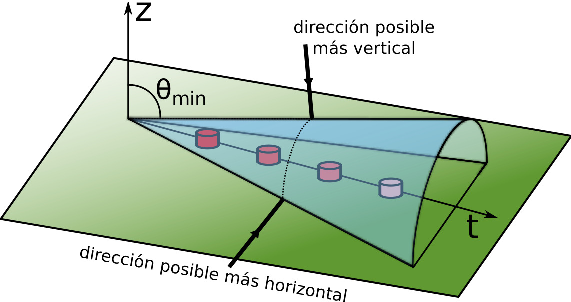
\includegraphics[width=0.75\textwidth]{fig/seleccionAuger/conoLineEvent.pdf}
	\caption{Esquema de reconstrucción geométrica de un evento en linea. Una cota mínima para el ángulo cenital se obtiene al considerar que el ángulo azimutal de la lluvia coincide con la linea que une las estaciones.}
	\label{fig:conoLineEvent}
	\end{center}
	\end{figure} 
	
	
	Este método se utiliza en las búsquedas de DGL y DGH.
	Dado que el problema esta mal condicionado para lluvias horizontales, no es posible utilizarlo en el analisis de ES.
	Para salvar este problema es necesario utilizar variables que no dependan de este tipo de ajuste, lo que se desarrolla en la siguiente sección.
	
	\subsection{Otras variables sensibles a la inclinación}
	
	Además de obtener una estimación directa del ángulo cenital $\theta$ a partir de un ajuste, es posible utilizar otro tipo de variables sensibles a la inclinación, como la velocidad aparente de la señal o la elongación de la huella sobre el detector.
	Mediante este tipo de variables es posible salvar las situaciones en las que la reconstrucción angular no puede ser llevada a cabo.
	Esta situación sucede muy frecuentemente para los neutrinos DGH casi horizontales y casi para la totalidad de los neutrinos ES.
	
		\subsubsection{Huella del evento}
		Los eventos inclinados tienden a producir una huella de señal elongada sobre el SD.
		Con el fin de cuantificar esta característica se construye un ``tensor de señal'':
		%
		\begin{eqnarray}
		S = \sum_i s_i, \quad \langle X \rangle = \sum_i s_i x_i/S, \quad \langle Y \rangle = \sum_i s_i y_i/S \nonumber \\
		I_{xx} = \sum_i s_i (x_i - \langle X \rangle)^2 / S, \quad I_{yy} = \sum_i s_i (y_i - \langle Y \rangle)^2 / S \nonumber \\
		I_{xy} = I_{yx} = \sum_i s_i (x_i - \langle X \rangle)(y_i - \langle Y \rangle) / S 
		\end{eqnarray}
		%
		Este objeto describe la distribución espacial de señal de misma forma en que el tensor de inercia, aplicado a un objeto extenso, lo hace con la masa.
		Continuando con esta analogía (ver figura \ref{fig:elipse}) se pueden obtener los ejes de la elipse de señal como:
		%
		\begin{eqnarray}
		L^2 =\frac{I_{xx}+I_{yy}+\sqrt{(I_{xx}-I_{yy})^2 + I_{xy}^2 }}{2S} \nonumber\\
		W^2 =\frac{I_{xx}+I_{yy}-\sqrt{(I_{xx}-I_{yy})^2 + I_{xy}^2 }}{2S} 
		\end{eqnarray}
		%
		Siendo $L$ la longitud del semieje mayor y $W$ la del menor (ver figura \ref{fig:elipse}).

		Como se discute en la sección \ref{sbsc:thetaRec}, es posible que una lluvia vertical junto con una estación accidental den como resultado un ángulo cenital reconstruido compatible con una cascada inclinada.
		Sin embargo, estos eventos no suelen presentar una huella elongada.
		De esta manera, el cociente $L/W$ puede usarse como criterio de calidad para eventos inclinados.
		
		\subsubsection{Velocidad aparente de la señal}
		En un evento inclinado genuino, el eje de la lluvia coincide con la dirección del semieje mayor de la elipse.
		Así, la velocidad aparente de la señal $V$ en ésta dirección permite obtener una buena aproximación del ángulo cenital.
		%
		\begin{equation}
		\sin\theta \simeq \frac{V}{c}
		\end{equation}
		%
		Para estimar $V$ a partir de un evento, se promedian las velocidades $V_{ij}\equiv L_{ij}/\Delta T_{ij}$ entre pares de estaciones cuya distancia, proyectada en la dirección del semieje mayor, sea superior a los \cant{1000}{mts} (ver panel derecho en la figura \ref{fig:elipse}).
		No se consideran los pares de estaciones con distancia $L_{ij}$ pequeñas ya que, producto de la propagación de la incerteza en el tiempo de disparo, presentan un error inaceptable en la velocidad de la señal estimada.
		%
		\begin{figure}[ht]
		\begin{center}
		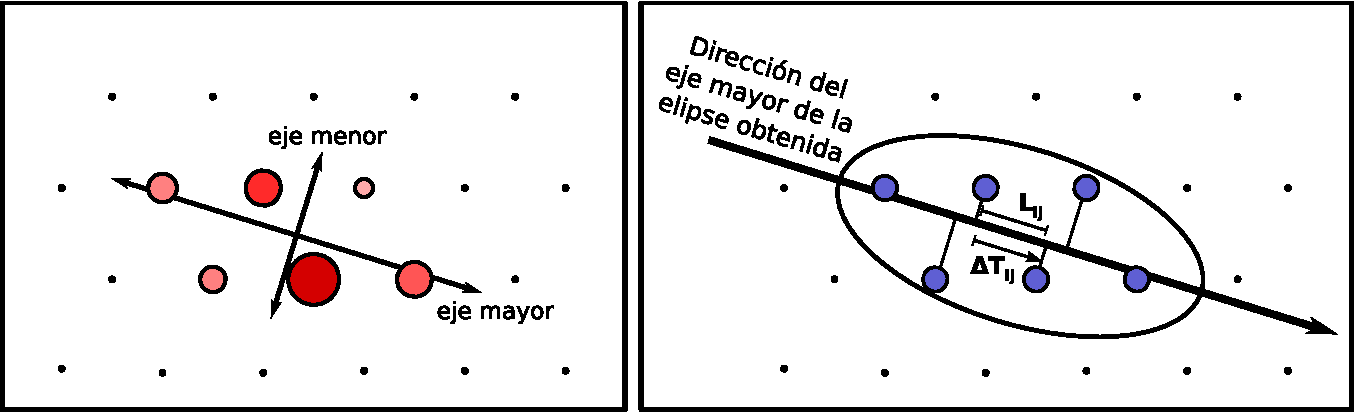
\includegraphics[width=1.0\textwidth]{fig/seleccionAuger/elipse.pdf}
		\caption{Diagrama de la elipse de señal que describe la configuración espacial de un evento inclinado (izquierda). Representación del cálculo de la velocidad de la señal en la dirección del semieje mayor (derecha).}
		\label{fig:elipse}
		\end{center}
		\end{figure}
		%
		
		\subsection{Desempeño de la selección de eventos inclinados}

\section{Selecci\'on de lluvias j\'ovenes}
	
	
	\section{Variables discriminantes}
	
	\section{Análisis multivariado}
	
	\section{Criterios de identificación}
	
		\subsection{Identificación de neutrinos DGL}
		
		\subsection{Identificación de neutrinos DGH}
		
		\subsection{Identificación de neutrinos ES}
	
	\begin{sidewaystable}[ht!]
	\begin{center}
		\renewcommand{\arraystretch}{1.4}
		\footnotesize
		\begin{tabular}{l|c|c|c}
		\hline
		Búsqueda & Earth-skimming (ES)           & Downward-going                        & Downward-going                       \\
				&                               & {\it high} angle (DGH)                & {\it low} angle (DGL)                \\
		\hline 
		Sabores e interacciones & $\nu_\tau$ CC & $\nu_e,~\nu_\mu~,\nu_\tau$ CC $\&$ NC &  $\nu_e,~\nu_\mu~,\nu_\tau$ CC $\&$ NC \\

		Rango angular & $\theta>90^\circ$             & $\theta \in (75^\circ, 90^\circ)$ & $\theta \in (60^\circ, 75^\circ)$ \\

		N$^\circ$ de estaciones(Nst) & Nst $\geq$ 3   & Nst $\geq$ 4 & Nst $\geq$ 4 \\
		\hline 
					& $-$                             & $\theta_{\rm rec}>$ 75$^{\circ}$   &   $\theta_{\rm rec}\in (58.5^\circ,~76.5^{\circ})$\\
		Lluvias    & $L/W > 5$                                         & $L/W > 3$ & $-$ \\
		Inclinadas & $\langle V\rangle\in (0.29,~0.31)~{\rm m~ns^{-1}}$ & $\langle V \rangle~<~0.313~{\rm m~ns^{-1}}$ & $-$ \\
				& RMS($V$)$~<~0.08~{\rm m~ns^{-1}}$                 & RMS($V$)/$\langle V\rangle<0.08$ & $-$ \\
		\hline 
				& Datos: 1 January 04 - 31 May 10 &                                     & $\geq 75\%$ de estaciones cercanas al   \\
				& $\geq 60\%$ of stations with  &                                      & core con ToT trigger       \\
		Lluvias     & ToT trigger \& AoP $>$ 1.4    & Discriminante de Fisher basado &                          \&        \\
		%\cline{2-2}
		Jóvenes   & Datos: 1 Junio 10 - 20 Junio 13   & en AoP estaciones {\it early}   & Discriminante de Fisher basado  \\
				& $\langle {\rm AoP} \rangle> 1.83$  &                                 & en AoP de las estaciones {\it early} \\
				& AoP$_{\rm min}$ $>$ 1.4 if Nst=3   &                                 & cercanas al core \\
		\hline
		\end{tabular}
		\vskip -3mm
		\caption{Resumen de los observables y valores numéricos de los cortes aplicados para seleccionar lluvias inclinadas y jóvenes en las tres búsquedas de neutrinos.} 
	\end{center}

	\label{tab:cuts}
	\end{sidewaystable}